\documentclass{beamer}
\usetheme{Darmstadt}
\usepackage{CJKutf8}

\usepackage[utf8]{inputenc}
\usepackage[OT1, T2A]{fontenc}
\usepackage{fontspec}
\usepackage[normalem]{ulem}

\usepackage{graphicx}
\usepackage{tikz}
\usepackage{braket}

\usepackage{xcolor}
\usepackage{pgfplots}
\usepackage{tikz}

\begin{document}

    \subsection{Background}
    \begin{frame}{SHA-256 Algorithm}
        This summary is heavily based on \cite{Fowler_2012}.
        \begin{itemize}
            \item Surface code is a method to construct \textit{logical} qubits from physical qubits with acceptable relativce error tolerance \cite{calderbank1997quantum}
            \item Logical qubits are more efficient than their physical counterparts
            \item The tolerance of surface codes to errors is high as about 1\%
            \item However, ensuring high tolerance requires massive physical qubits and sequential Toffoli gates
            \begin{itemize}
                \item ``We assume an error rate approximately one-tenth the threshold rate, which implies that we need about 14,500 physical qubits per logical qubit to give a sufficiently low logical error rate to successfully execute the algorithm"
            \end{itemize}
        \end{itemize}
    \end{frame}
    
    \begin{frame}[t]{Surface code and physical qubits}
        \begin{itemize}
            \item However, ensuring high tolerance requires massive physical qubits and sequential Toffoli gates
            \begin{itemize}
                \item ``A much larger part of the surface code is however needed to generate and purify the special ancilla $\ket{A_L}$ states that are used in the Toffoli gates."
                \item Applying Shor's Algorithm to 2,000-bit integer requires $ 2.2 \times 10^{12} \ket{A_L}$ states and takes about 26.7 hours
                \item The surface code needs to generate these states in a timely manner
            \end{itemize}
        \end{itemize}
    \end{frame}
    
    \begin{frame}[t]{Surface code and physical qubits}
        \begin{itemize}
            \item However, ensuring high tolerance requires massive physical qubits and sequential Toffoli gates
            \begin{itemize}
                \item ``We assume an error rate approximately one-tenth the threshold rate, which implies that we need about 14,500 physical qubits per logical qubit to give a sufficiently low logical error rate to successfully execute the algorithm"
                \item In result, 58 million qubits are required for computation
                \item Additionally 1 billion qubits are required for generating $\ket{A_L}$ states
            \end{itemize}
            \item Hopefully, ``the size of the quantum computer is quite sensitive tothe error rate in the physical qubits.''
            \begin{itemize}
                \item ``For example, improving the overall error rate by about a factor of ten, as detailed in Appendix M, can reduce the number of physical qubits by about an order of magnitude, to about 130 million, although leaving the execution time unchanged.''
            \end{itemize} 
        \end{itemize}
    \end{frame}
    
    \subsection{Introduction}
    \begin{frame}{Qubit operators}
        Quantum computation is based on qubits: two-level quantum systems
        \begin{itemize}
            \item Based on quantum physics and election spins
        \end{itemize}
        These electron spins can be reprensented by various operators such as Pauli-X, Y, Z operators.
    \end{frame} 
           
    \begin{frame}{Qubit operators}
        Basic recap of Pauli operators and qubit operators:
        \begin{itemize}
            \item Ground state for $\shat{Z}$ axis : $\ket{g} = \begin{pmatrix} 1 \\ 0 \end{pmatrix}$
            \item Excited state : $\ket{e} = \begin{pmatrix} 0 \\ 1 \end{pmatrix}$
            \item $\shat{Z} = \hat{\sigma_z} = \begin{pmatrix}
            1 & 0 \\
            0 & -1
            \end{pmatrix}$, with eigenvalues $+1$ and $-1$ for $\ket{g}$, $ \ket{e} $.
            \item $\shat{X} = \hat{\sigma_x} = \begin{pmatrix}
            0 & 1 \\
            1 & 0
            \end{pmatrix}$, with eigenvalues $+1$ and $-1$ for $\ket{+} = \frac{1}{\sqrt{2}}\begin{psmallmatrix} 1 \\ 1 \end{psmallmatrix} = \frac{1}{\sqrt{2}}(\ket{g} + \ket{e})$, $\ket{-} = \frac{1}{\sqrt{2}}\begin{psmallmatrix} 1 \\ -1 \end{psmallmatrix} = \frac{1}{\sqrt{2}}(\ket{g} - \ket{e})$.
            \item $\shat{Y} = -i\hat{\sigma_y} = \shat{Z}\shat{X} = \begin{pmatrix}
            0 & 1 \\
            -1 & 0
            \end{pmatrix}$, which is real unlike $ \hat{\sigma_y} $.
        \end{itemize}
    \end{frame}
    
    \begin{frame}{Qubit operators}
        These qubit operators satisfy the following:
        \begin{equation}
        \begin{split}
            \shat{X}\,^2 &= -\shat{Y}\,^2 = \shat{Z}\,^2 = I \\
            \shat{X}\shat{Z} &= -\shat{Z}\shat{X} \\
            [\shat{X},\shat{Y}] &= \shat{X}\shat{Y} - \shat{Y}\shat{X} = -2\shat{Z}
        \end{split}
        \label{eq:quant_op}
        \end{equation}
        Also note that each measurement based on each quantum operators yields one of its eigenstates. For example, $M_Z$ will return $ \ket{g} $ or $ \ket{e} $, while $ M_X $ will return $ \ket{+} $ or $ \ket{-} $.
    \end{frame}
    
    \begin{frame}{Qubit operators}
        \begin{itemize}
            \item Any two-level quantum system that satisfies (\ref{eq:quant_op}) can be used as a qubit.
            \item There are infinitely many quantum states...
            \item Hopefully, Solovay–Kitaev theorem states that an arbitrary quantum gate can be approximated by a reasonably short sequence of universial gates.
            \begin{itemize}
                \item An $m$ constant qubit gate can be approximated to an $ \epsilon $-error by $ \mathcal{O}(m \log^c(m/\epsilon)) $ for some $ c $.
            \end{itemize}
            \item One of the common quantum universial gate set is `Clifford + T' gate set: CNOT, $ \shat{H} $(Hadamard gate), $ \shat{S} $ and $ \shat{T} $.\footnote{$ T^4 = S^2 = Z = R_\pi$, where $ R_\theta = \begin{psmallmatrix}
            1 & 0 \\
            0 & e^{i\theta}
            \end{psmallmatrix} $.}
        \end{itemize}
    \end{frame}
    

    \begin{frame}{Single-qubit errors}
        Qubits errors are random $ \shat{X} $ bit-flip and/or $ \shat{Z} $ phase-flip.
        \begin{itemize}
            \item These single-qubit errors can be undone after detection
            \begin{itemize}
                \item Erroneous $ \shat{Z} $ can be cancelled with another $ \shat{Z} $ since $ \shat{Z}^2 = I $
            \end{itemize}
            \item Also, applying qubit operation does not alter the probability of its eigenstate
        \end{itemize}
        Thus detection, rather than correction, is the key point of surface code.
    \end{frame}
    
    \begin{frame}{Single-qubit errors}
        \begin{itemize}
            \item However since $ [\shat{X}, \shat{Z}] \neq \hat{0} $, sequential measurements of $ \shat{X} $ and $ \shat{Z} $ might conflict each other (since $ \shat{X}\shat{Z} \neq \shat{Z}\shat{X} $).
            \item This problem can be avoided by measuring multi-qubits at once. Consider qubit $ a $ and $ b $ and operation $ \sshat{X_a}\sshat{X_b} $ and $ \sshat{Z_a}\sshat{Z_b} $, then these two operations do commute!
        \end{itemize}
        \begin{equation}
        \begin{split}
        [\sshat{X_a}\sshat{X_b}, \sshat{Z_a}\sshat{Z_b}] &= (\sshat{X_a}\sshat{X_b})(\sshat{Z_a}\sshat{Z_b}) - (\sshat{Z_a}\sshat{Z_b})(\sshat{X_a}\sshat{X_b}) \\
        &= \sshat{X_a}\sshat{Z_a}\sshat{X_b}\sshat{Z_b} - \sshat{Z_a}\sshat{X_a}\sshat{Z_b}\sshat{X_b} \\
        &= (-\sshat{Z_a}\sshat{X_a})(-\sshat{Z_b}\sshat{X_b}) - (\sshat{Z_a}\sshat{X_a})(\sshat{Z_b}\sshat{X_b}) \\
        &= \hat{0}
        \end{split}
        \end{equation}
        Therefore $ \sshat{X_a}\sshat{X_b} $ and $ \sshat{Z_a}\sshat{Z_b} $ can be used as basis of 2-qubit system.
    \end{frame}
    
    \begin{frame}{Single-qubit errors}
        In this case, the following are the (entangled) eigenstates, which does not change its state after measurements by $ \sshat{X_a}\sshat{X_b} $ or $ \sshat{Z_a}\sshat{Z_b} $.
        \begin{table}[h]
            \begin{tabular}{|c|c|c|}
                \hline
                $ \sshat{Z_a}\sshat{Z_b} $ & $ \sshat{X_a}\sshat{X_b} $ & $ \ket{\psi} $ \\ \hline
                $ +1 $ & $ +1 $ & $ (\ket{gg} + \ket{ee})/\sqrt{2} $ \\ \hline
                $ +1 $ & $ -1 $ & $ (\ket{gg} - \ket{ee})/\sqrt{2} $ \\ \hline
                $ -1 $ & $ +1 $ & $ (\ket{ge} + \ket{eg})/\sqrt{2} $ \\ \hline
                $ -1 $ & $ -1 $ & $ (\ket{ge} - \ket{eg})/\sqrt{2} $ \\ \hline
            \end{tabular}
        \end{table}
        For example, if $ \ket{\psi} = (\ket{gg} - \ket{ee})/\sqrt{2}$, then $ \sshat{Z_a}\sshat{Z_b}\ket{\psi} = \ket{\psi} $ and $ \sshat{X_a}\sshat{X_b}\ket{\psi} = -\ket{\psi} $ since $ (+1, -1) $ are its eigenvalues.
    \end{frame}
    
    \begin{frame}{Single-qubit errors}
        If there is an random $ \shat{X} $ or $ \shat{Z} $ error on a single qubit, the original eigenstate will change into another eigenstate.
        \begin{itemize}
            \item If $ \ket{\psi} = (\ket{gg} - \ket{ee})/\sqrt{2}$, then $ \sshat{X_a}\ket{psi} = -(\ket{ge} - \ket{eg})/\sqrt{2}$, where eigenvalues changed to $ (-1, -1) $.
            \item However, $ \sshat{X_b}\ket{psi}$ also yields $ -(\ket{ge} - \ket{eg})/\sqrt{2}$
            \item Errors can be detected, but cannot be uniqlely identified
            \item A simple form of error detection code
        \end{itemize}
        Operator products such as $ \sshat{X_a}\sshat{X_b} $ or $ \sshat{Z_a}\sshat{Z_b} $ are called stabilizers
        \begin{itemize}
            \item Eigenstates are measureable without any quantum information loss
        \end{itemize}
    \end{frame}
    
    \subsection{Surface Code}
    \begin{frame}{Surface code structure}
        The following figure is the implementation of the surface code on a two-dimensional array of physical qubits.
        
        \begin{minipage}[0.65\textheight]{\textwidth}
        \begin{columns}[T]
            \begin{column}{0.4\textwidth}
                \begin{figure}[h]
                    \centering
                    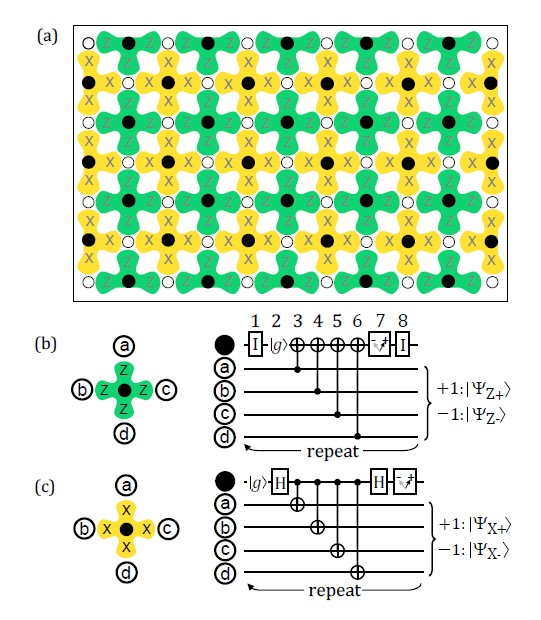
\includegraphics[height=0.6\textheight]{./Images/surf-code-overview.jpg}
                \end{figure}
            \end{column}
            \begin{column}{0.6\textwidth}
                \only<1>{
                    \begin{itemize}
                    \item The open circles are \textit{data qubits} where the computational quantum states are stored.
                    \item The filled circles are \textit{measurement qubits}.
                    \item These qubits should be able to perform initialization, single-qubit rotation, CNOT between neighbors, SWAP and $ M_Z $.
                    \end{itemize}
                }
                \only<2>{
                    \begin{itemize}
                        \item Measurement qubits are used to stabilize and alter the quantum state of data qubits
                        \begin{itemize}
                            \item Two types exist: ``measure-Z'' qubits (colored in green) and ``measure-X'' qubits (colored in yellow)
                        \end{itemize}
                        \item Each data qubits are connected to two measure-Z qubits and measure-X qubits
                    \end{itemize}
                }
                \only<3>{
                    \begin{itemize}
                        \item Measurement qubits either measures $ \shat{X} $ or $ \shat{Z} $ stabilizer (i.e., $ \sshat{X_a}\sshat{X_b}\sshat{X_c}\sshat{X_d} $ or $ \sshat{Z_a}\sshat{Z_b}\sshat{Z_c}\sshat{Z_d} $)
                        \item Figure (b) and (c) represents the quantum circuit of stabilizer measurement
                        \item For any adjacent data qubits with state $ \ket{\psi} $, $ \sshat{X_a}\sshat{X_b}\sshat{X_c}\sshat{X_d}\ket{\psi} = X_{abcd}\ket{\psi } $ holds.
                        \item After measurement, the cycle is repeated (to negate the effects)
                    \end{itemize}
                }
            \end{column}
        \end{columns}
        
        \end{minipage}
        
    \end{frame}
    

    \subsection{Quinscent State}
    \begin{frame}{Surface code structure}
        \begin{minipage}[0.65\textheight]{\textwidth}
        \begin{columns}[T]
            \begin{column}{0.4\textwidth}
                \begin{figure}[h]
                    \centering
                    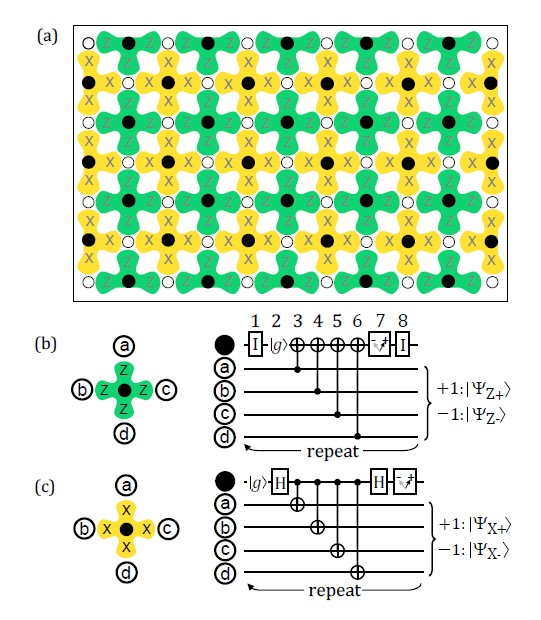
\includegraphics[height=0.6\textheight]{./Images/surf-code-overview.jpg}
                \end{figure}
            \end{column}
            \begin{column}{0.6\textwidth}
                    \begin{itemize}
                    \item The techniques used to apply $ \sshat{X_a}\sshat{X_b}\sshat{X_c}\sshat{X_d} $ and $ \sshat{Z_a}\sshat{Z_b}\sshat{Z_c}\sshat{Z_d} $ are somewhat standard, but is surely crucial.
                    \item On (b), identity matrix is included in measure-Z to minimize error and match timing with measure-X.
                    \end{itemize}
            \end{column}
        \end{columns}
        
        \end{minipage}
        
    \end{frame}
    \begin{frame}{Quinscent state}
        \begin{itemize}
            \item The forementions state $ \ket{\psi} $ is not the ground state $ \ket{g} $
            \item Instead it is determined by its eigenvectors
            \item The data qubits are projected to these states
            \item They are not fully entangled to all of the qubits, but are locally entangled
        \end{itemize}
    \end{frame}
    
    %
    \subsection{Single-qubit Errors}
    \begin{frame}{Single-qubit error in a nutshell}
        \begin{figure}[h]
            \centering
            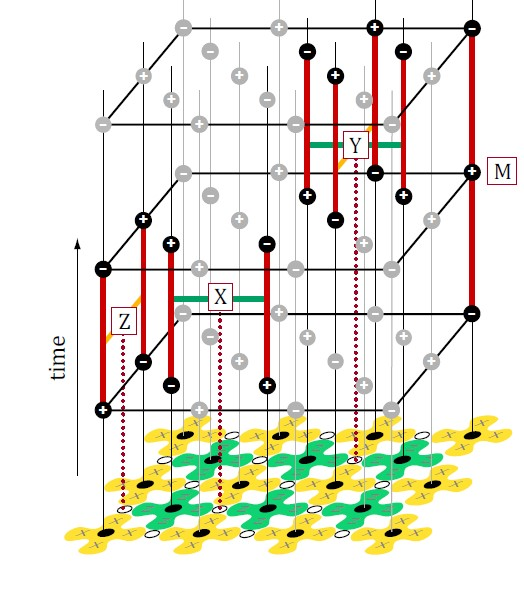
\includegraphics[height=0.8\textheight]{./Images/surf-code-single-error.jpg}
        \end{figure}
    \end{frame}
    
    \begin{frame}{Single phase-flip error}
        Consider a random $ \shat{Z} $ phase-flip error $ \sshat{I_a} + \epsilon \sshat{Z_a} $ where $ \lvert\epsilon\rvert \ll 1 $. Let $ \ket{\psi'} \to (\sshat{I_a} + \epsilon \sshat{Z_a}) \ket{\psi} $, then $ \ket{\psi'} = \sshat{Z_a}\ket{\psi} $ with probability $ \lvert\epsilon\rvert^2 $.
        \begin{equation}
        \begin{split}
       \sshat{X_a}\sshat{X_b}\sshat{X_c}\sshat{X_d}(\sshat{Z_a} \ket{\psi}) &= -\sshat{Z_a}(\sshat{X_a}\sshat{X_b}\sshat{X_c}\sshat{X_d}\ket{\psi}) \\
       &= -\sshat{Z_a}X_{abcd}\ket{\psi}
        \end{split}
        \end{equation}
        Thus, a single $ \shat{Z} $ phase-flip error can be detected by measure-X with any info loss since $ \ket{\psi} $ is the eigenstate of stabilizers $ \sshat{X_a}\sshat{X_b}\sshat{X_c}\sshat{X_d} $ and $ \sshat{Z_a}\sshat{Z_b}\sshat{Z_c}\sshat{Z_d} $. However, it will not change the result of measure-Z.
        \begin{equation}
        \begin{split}
       \sshat{Z_a}\sshat{Z_b}\sshat{Z_c}\sshat{Z_d}(\sshat{Z_a} \ket{\psi}) &= \sshat{Z_a}(\sshat{Z_a}\sshat{Z_b}\sshat{Z_c}\sshat{Z_d}\ket{\psi}) \\
       &= \sshat{Z_a}Z_{abcd}\ket{\psi}
        \end{split}
        \end{equation}
    \end{frame}
    
    \begin{frame}{Other errors}
        \begin{itemize}
            \item We can apply $ \sshat{Z_a} $ to negate this error, but applying another quantum operator may yield other errors
            \item Marking that the qubit is phase-flipped by software is better
            \item Similarly, a single $ \shat{X} $ bit-flip error can be detected by measure-Z.
        \end{itemize}
        Measurement can also yield errors, which has to be considered.
        \begin{itemize}
            \item However, it is very unlikely to happen twice in a row or more
            \item Even so, several measurements are required to ensure the result
        \end{itemize}
    \end{frame}
    
    \begin{frame}{Single-qubit error in a nutshell (recap)}
        \begin{figure}[h]
            \centering
            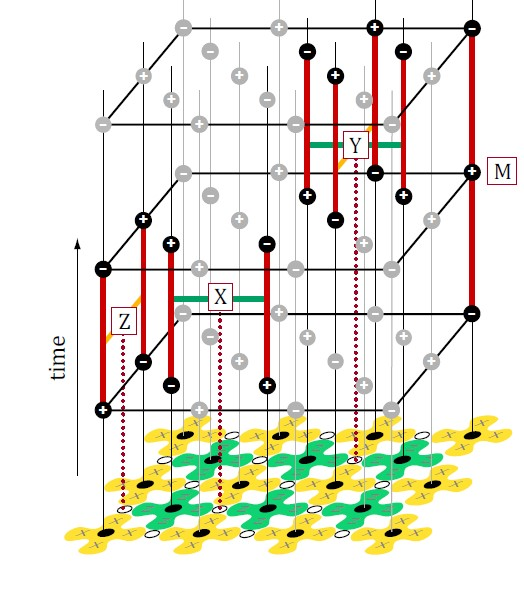
\includegraphics[height=0.7\textheight]{./Images/surf-code-single-error.jpg}
        \end{figure}
        Vertical heavy lines indicate each errors
    \end{frame}
    
    \subsection{Logical Operators}
    \begin{frame}{Logical operators in a nutshell}
        \begin{figure}
            \centering
            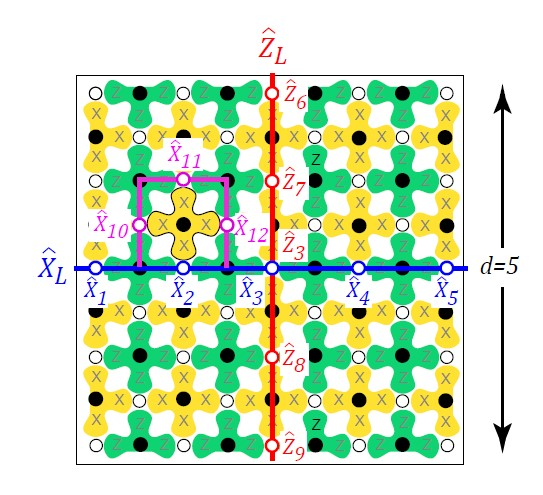
\includegraphics[height=0.6\textheight]{./Images/surf-code-logical.jpg}
        \end{figure}
        $ \sshat{X_L} $ and $ \sshat{Z_L} $ can manipulate qubits without altering the measurement results.
    \end{frame}

    \begin{frame}{9 by 9 surface code}
        \begin{minipage}[0.65\textheight]{\textwidth}
        \begin{columns}[T]
            \begin{column}{0.4\textwidth}
                \begin{figure}[t]
                    \centering
                    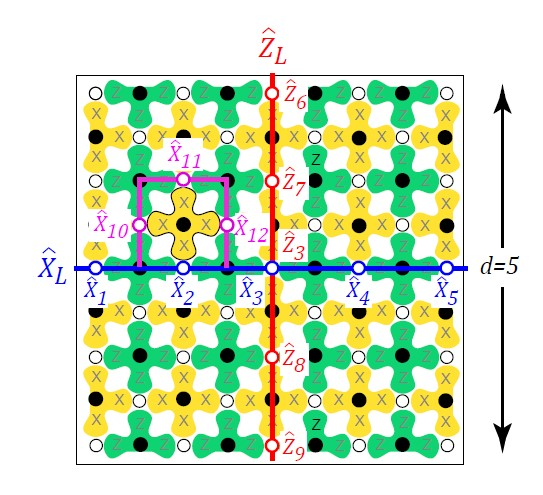
\includegraphics[height=0.6\textheight]{./Images/surf-code-logical.jpg}
                \end{figure}
            \end{column}
            \begin{column}{0.6\textwidth}
                \begin{itemize}
                \item This 9 by 9 surface code contains 41 data qubits and 40 measurement qubits
                \begin{itemize}
                    \item Thus there are 2 $ \times $ 41 degrees of   freedom and 2 $ \times $ 40 constraints with the stabilizer
                    \item All of these constraints are linearly independent
                \end{itemize}
                \item Where are the remaining two unconstrained degrees of freedom? How can we manipulate those?
                \end{itemize}
            \end{column}
        \end{columns}
        \end{minipage}
    \end{frame}
    
    \begin{frame}{9 by 9 surface code}
        \begin{itemize}
            \item A single data qubit $ \shat{X} $ operation only alters the measure-Z outcomes on either side
            \begin{itemize}
                \item As mentioned, all $ \sshat{X_i} $ operations mutually commute.
            \end{itemize}
            \item However, two simultaneous $ \shat{X} $ operations on two data qubits $ a $ and $ b $ that both neighbor the same measure-$ Z $ qubit commutes with the $ \shat{Z} $ stabilizer
            \item As a formula, $ [\sshat{Z_a}\sshat{Z_b}\sshat{Z_c}\sshat{Z_d}, \sshat{X_a}\sshat{X_b}] = 0$.
        \end{itemize}
    \end{frame}
    
    \begin{frame}{9 by 9 surface code}
        \begin{minipage}[0.65\textheight]{\textwidth}
        \begin{columns}[T]
            \begin{column}{0.4\textwidth}
                \begin{figure}[t]
                    \centering
                    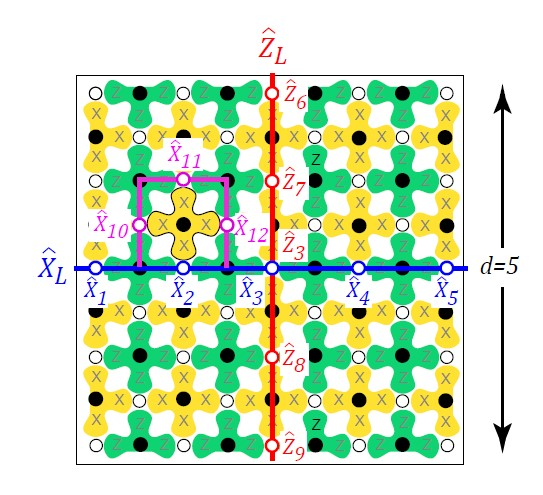
\includegraphics[height=0.6\textheight]{./Images/surf-code-logical.jpg}
                \end{figure}
            \end{column}
            \begin{column}{0.6\textwidth}
                \begin{itemize}
                \item We first apply $ \sshat{X_1} $. To negate the measure-Z, we also apply $ \sshat{X_2} $, and so on.
                \item Thus, $ \sshat{X_L} = \sshat{X_1}\sshat{X_2}\sshat{X_3}\sshat{X_4}\sshat{X_5} $ commutes with any stabilizer.
                \item $ \ket{\psi_X} = \sshat{X_L} \ket{\psi} $ is different from $ \ket{\psi} $, but its measurement will yield $ \ket{\psi} $.
                \end{itemize}
            \end{column}
        \end{columns}
        \end{minipage}
    \end{frame}
    
    \begin{frame}{9 by 9 surface code}
        \begin{minipage}[0.65\textheight]{\textwidth}
        \begin{columns}[T]
            \begin{column}{0.4\textwidth}
                \begin{figure}[t]
                    \centering
                    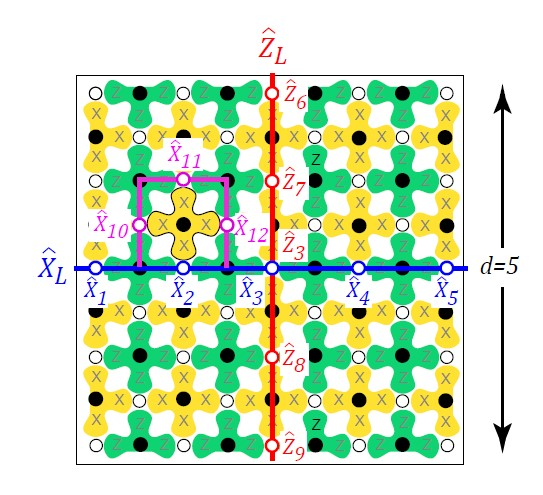
\includegraphics[height=0.6\textheight]{./Images/surf-code-logical.jpg}
                \end{figure}
            \end{column}
            \begin{column}{0.6\textwidth}
                \begin{itemize}
                \item Since $ \sshat{X_L} $ cannot be written as a product of stabilizers, this operator manipulates one of the unconstrained degrees of freedom.
                \item Similarly $ \sshat{Z_L} = \sshat{Z_6}\sshat{Z_7}\sshat{Z_3}\sshat{Z_8}\sshat{Z_9}$ manipulates the other degree of freedom.
                \item Are there any other methods to manipulate unconstrained degrees of freedom other than $ \sshat{X_L} $ and $ \sshat{Z_L} $? No!
                \end{itemize}
            \end{column}
        \end{columns}
        \end{minipage}
    \end{frame}
    
    \begin{frame}{9 by 9 surface code}
        \begin{minipage}[0.65\textheight]{\textwidth}
        \begin{columns}[T]
            \begin{column}{0.4\textwidth}
                \begin{figure}[t]
                    \centering
                    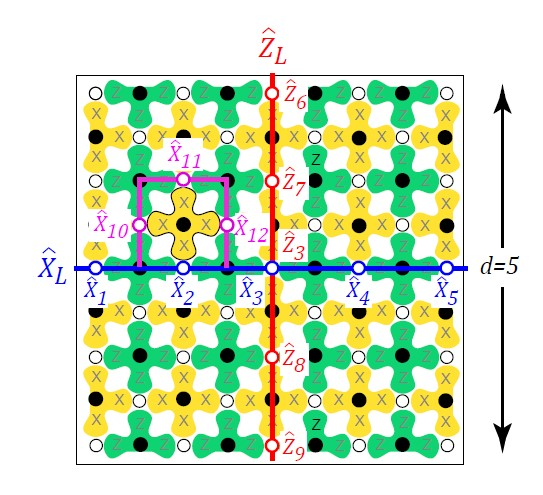
\includegraphics[height=0.6\textheight]{./Images/surf-code-logical.jpg}
                \end{figure}
            \end{column}
            \begin{column}{0.6\textwidth}
                \begin{itemize}
                \item Consider $ \sshat{X'_L} = \sshat{X_1}\shat{X_{10}}\sshat{X_{11}}\sshat{X_{12}}\sshat{X_3}\sshat{X_4}\sshat{X_5} $
                \item It might be a new chain, but is actually $ (\sshat{X_2}\shat{X_{10}}\sshat{X_{11}}\sshat{X_{12}})\sshat{X_L} $.
                \begin{itemize}
                    \item Since it is merely a product of $ \sshat{X_L}  $ and a stabilizer 
                \end{itemize}
                \item The same is applied to $ \sshat{Z_L} $; therefore there are no linearly independent operators other than $ \sshat{X_L} $ and $ \sshat{Z_L} $.
                \end{itemize}
            \end{column}
        \end{columns}
        \end{minipage}
    \end{frame}
    
    \begin{frame}{9 by 9 surface code : Conclusion}
        \begin{itemize}
            \item Thus quinscent state $ \ket{\psi} $ can be written as $ \ket{Q}\ket{q_L} $
            \begin{itemize}
                \item $ \ket{Q} $ is the vector of $ 2^N $-dimensional Hilbert space by $ N $ stabilizer measurements
                \item $ \ket{q_L} $ is a vector of $ 2 $-dimensional Hilbert space, representing unconstrained degrees of freedom
            \end{itemize}
            \item Stabilizers only affect $ \ket{Q} $ while $ \sshat{X_L} $ and $ \sshat{Z_L} $ only affect $ \ket{q_L} $
            \item Therefore a single logical qubit is constructed.
        \end{itemize}
        How to create more degrees of freedom?
    \end{frame}
    

\end{document}